
\ssn{Example continued}
For \S\ref{w1ss}, part (a) above we could instead think in stages. The probability of the first toss being H is $1/2$. The probability of the second toss also being H is $1/2$ and so the probability of the first two being a head is $(1/2)\times(1/2) = 1/4$. Finally, the probability of the third toss also being H is $1/2$ and so the probability of all three being H is $(1/2)^3 = 1/8$. 

We can sum this calculation up in a \emph{probability tree}:

\tikzset{
  treenode/.style = {shape=rectangle, rounded corners,
                     draw, align=center,
                     top color=white, bottom color=blue!30},
  root/.style     = {treenode, font=\Large, bottom color=red!30},
  env/.style      = {treenode},
  branch/.style = {treenode, bottom color=blue!10},  
  dummy/.style    = {circle,draw}
}
\tikzstyle{level 1}=[level distance=3.5cm, sibling distance=3.5cm]
\tikzstyle{level 2}=[level distance=3.5cm, sibling distance=2cm]

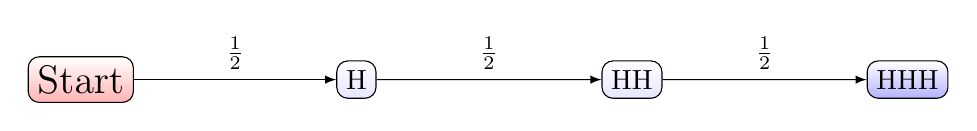
\begin{tikzpicture}
[
grow=right,
    edge from parent/.style = {draw, -latex},
    every node/.style       = {font=\normalsize}
  ]
\node[root]{Start}
child {
    node[branch]{H}
    child {
        node[branch]{HH}
        child {
            node[env]{HHH}
            edge from parent node[above] {$\frac{1}{2}$}                      }
        edge from parent node[above] {$\frac{1}{2}$}
        }                
    edge from parent node[above] {$\frac{1}{2}$}        
    }  ;           
\end{tikzpicture}

You may feel this tree has fewer branches than a good tree should have. Of course, other things could happen along the way which we have omitted. All the branches appear in the full tree below. 

\tikzstyle{level 1}=[level distance=3.5cm, sibling distance=5.0cm]
\tikzstyle{level 2}=[level distance=3.5cm, sibling distance=2.5cm]
\tikzstyle{level 3}=[level distance=3.5cm, sibling distance=1.3cm]

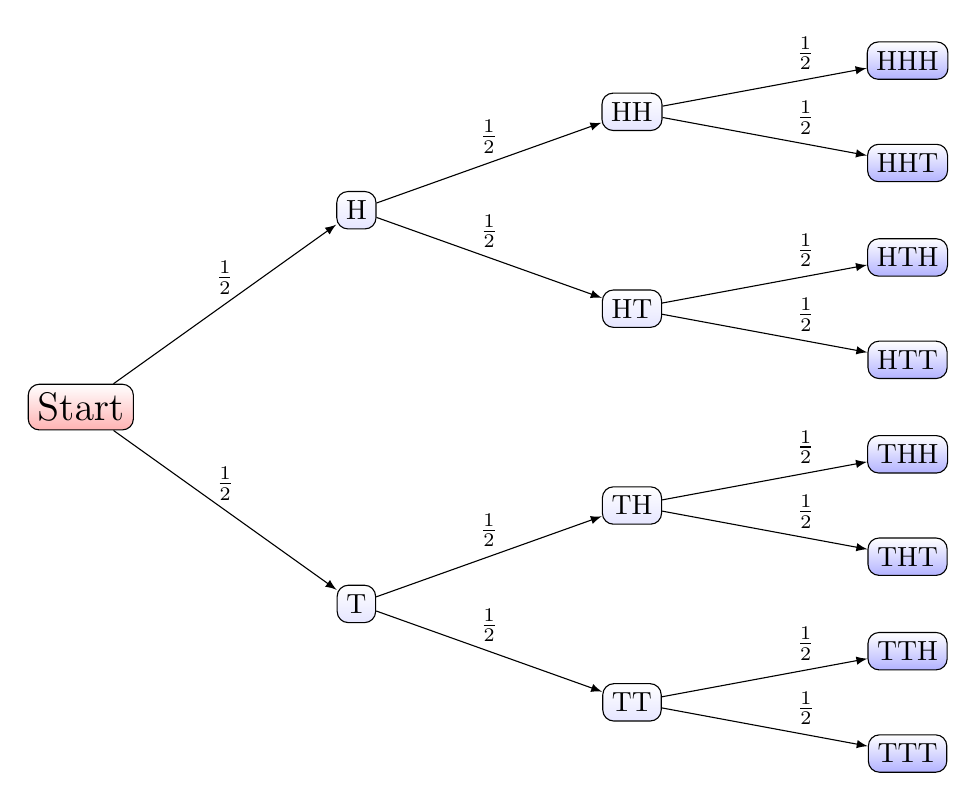
\begin{tikzpicture}
[
grow=right,
    edge from parent/.style = {draw, -latex},
    every node/.style       = {font=\normalsize}
  ]
\node[root]{Start}
child { 
    node[branch]{T}
    child { 
        node[branch]{TT}
        child{ 
             node[env]{TTT}
             edge from parent node[above,pos=0.7]{$\frac{1}{2}$}                    }
        child{ 
             node[env]{TTH}
             edge from parent node[above,pos=0.7]{$\frac{1}{2}$}      
             }               
        edge from parent node[above]{$\frac{1}{2}$} 
        }       
    child { 
        node[branch]{TH}
        child{ 
             node[env]{THT}
             edge from parent node[above,pos=0.7]{$\frac{1}{2}$}                    }
        child{ 
             node[env]{THH}
             edge from parent node[above,pos=0.7]{$\frac{1}{2}$}      
             }               
        edge from parent node[above]{$\frac{1}{2}$} 
        }       
    edge from parent node[above]{$\frac{1}{2}$}            
    }
child { 
    node[branch]{H}
    child { 
        node[branch]{HT}
        child{ 
             node[env]{HTT}
             edge from parent node[above,pos=0.7]{$\frac{1}{2}$}                    }
        child{ 
             node[env]{HTH}
             edge from parent node[above,pos=0.7]{$\frac{1}{2}$}      
             }               
        edge from parent node[above]{$\frac{1}{2}$} 
        }       
    child { 
        node[branch]{HH}
        child{ 
             node[env]{HHT}
             edge from parent node[above,pos=0.7]{$\frac{1}{2}$}                    }
        child{ 
             node[env]{HHH}
             edge from parent node[above,pos=0.7]{$\frac{1}{2}$}      
             }               
        edge from parent node[above]{$\frac{1}{2}$} 
        }       
    edge from parent node[above]{$\frac{1}{2}$}            
    }     ;           
\end{tikzpicture}
\end{n}

\ssn{Example}
A six-sided die (``D6'' for short) is a gadget that produces each of the results 1,2,3,4,5,6 with equal probability. 
Which is more likely: rolling two D6 and obtaining 6 both times or tossing five coins and all of them coming down H? 

The probability of two 6's is $(1/6)^2= 1/36$.   The probability of five out of five heads is $(1/2)^5 = 1/32$.  So the coins coming up heads is more likely. 
\end{n}

\ssn{Definition} 
If an experiment produces an outcome which is equally likely to be any element of a finite sample space $S$, we say that an element of $S$ is chosen \emph{uniformly randomly}. 

For example, a single roll of a D6 is choosing an element of $\{ 1,2,3,4,5,6\}$ uniformly randomly. 
\end{n}
 
\ssn{Another tree example} 
An ``$n$-sided die'' is a real or imaginary object that chooses an element of $\{ 1,2,\dots, n \}$ uniformly randomly.  We will call such a thing a ``D$n$''. You can buy a D$n$ for many values of $n$ in gaming shops. 

Player A rolls a D3 and player B rolls a D4 and the winner is the person who rolls the higher number. In this rather unfair game, what are the probabilities that player A wins, draws and loses?   We will draw a tree, imagining that A rolls first. We will write $a$ for A's roll. Note how the labels on the arrows emerging from a node add up to $1$.  

\tikzset{
  treenode/.style = {shape=rectangle, rounded corners,
                     draw, align=center,
                     top color=white, bottom color=blue!20},
  root/.style     = {treenode, font=\Large, bottom color=red!30},
  env/.style      = {treenode},
  branch/.style = {treenode, bottom color=blue!10},  
  dummy/.style    = {circle,draw}
}
\tikzstyle{level 1}=[level distance=3.0cm, sibling distance=4.5cm]
\tikzstyle{level 2}=[level distance=8.5cm, sibling distance=1.5cm]
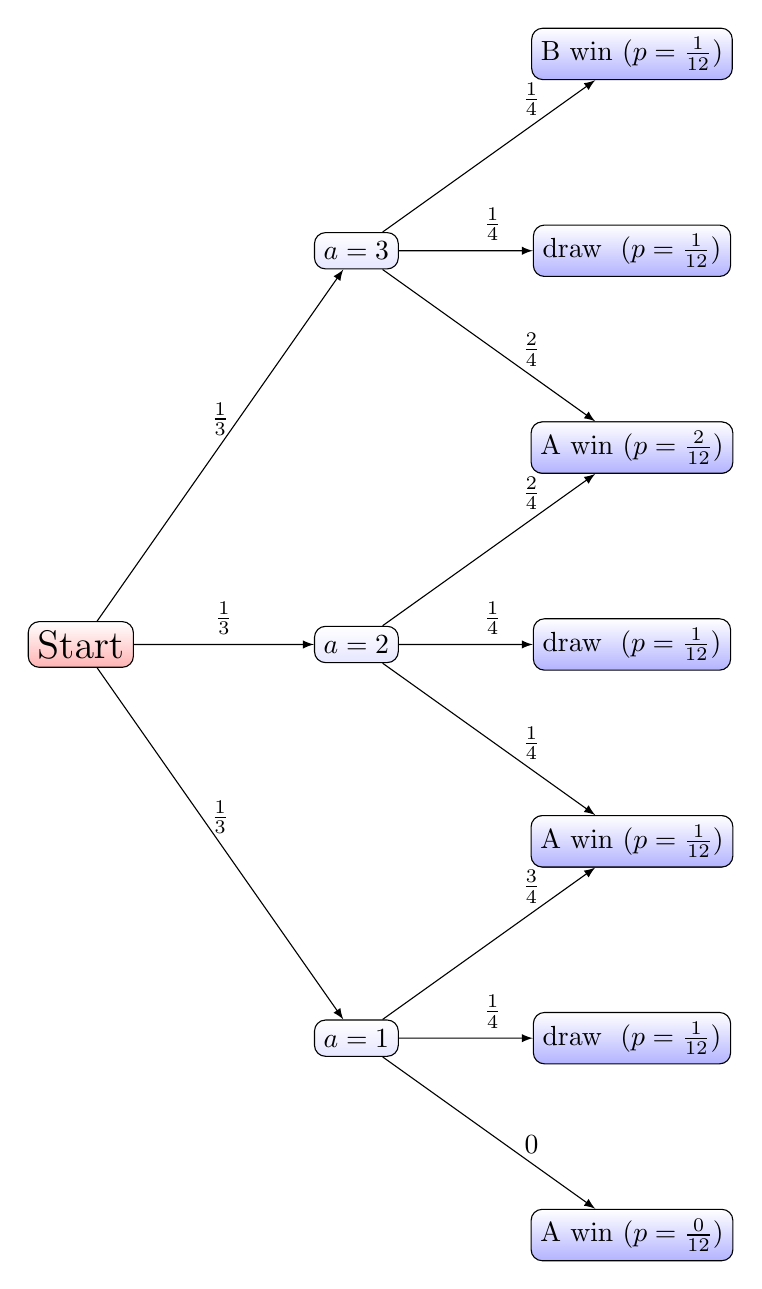
\begin{tikzpicture}
  [
    grow                    = right,
    edge from parent/.style = {draw, -latex},
    every node/.style       = {font=\normalsize}
  ]
\node[root]{Start}
child {
    node[branch]{$a=1$}
    child {
        node[env]{A win $(p=\frac{0}{12})$}
        edge from parent node[above,pos=0.7] {$0$}
        }
        child {
        node[env]{draw~~$(p=\frac{1}{12})$}
        edge from parent 
        node[above,pos=0.7] {$\frac{1}{4}$}
        }
       child {
        node[env]{B win $(p=\frac{3}{12})$}
        edge from parent 
        node[above,pos=0.7] {$\frac{3}{4}$}
        }  
    edge from parent 
    node[above] {$\frac{1}{3}$}
    }
    child {
    node[branch]{$a=2$}
    child {
        node[env]{A win  $(p=\frac{1}{12})$}
        edge from parent 
        node[above,pos=0.7] {$\frac{1}{4}$}
        }
        child {
        node[env]{draw~~$(p=\frac{1}{12})$}
        edge from parent 
        node[above,pos=0.7] {$\frac{1}{4}$}
        }    
        child {
        node[env]{B win $(p=\frac{2}{12})$}
        edge from parent 
        node[above,pos=0.7] {$\frac{2}{4}$}
        }    
    edge from parent 
    node[above] {$\frac{1}{3}$}
    }
    child {
    node[branch]{$a=3$}
    child {
        node[env]{A win $(p=\frac{2}{12})$}
        edge from parent 
        node[above,pos=0.7] {$\frac{2}{4}$}
        }
        child {
        node[env]{draw~~$(p=\frac{1}{12})$}
        edge from parent 
        node[above,pos=0.7] {$\frac{1}{4}$}
        }   
        child {
        node[env]{B win $(p=\frac{1}{12})$}
        edge from parent 
        node[above,pos=0.7] {$\frac{1}{4}$}
        }   
    edge from parent 
    node[above] {$\frac{1}{3}$}
    };           
\end{tikzpicture}


You should check all the calculations. As an example, near the top there is an edge labelled ``$2/4$'' that leads to a win for A.  What that means is that \emph{if we know that A has rolled a 3}, then the probability that A wins is $2/4 = 1/2$. This is true because when $a=3$, A wins if B rolls a 1 or 2 but draws or loses if B rolls 3 or 4. 

The probability of G happening given that we already know that H has happened is called a \emph{conditional probability} and written $\PP( G | H)$. It is often abbreviated to ``the probability of G given H''. Thus we could write 
 \[
\PP(\text{A wins} \st a=3) = 2/4 = 1/2.
 \]

At the end of the ``$a=3$'' branch, a probability of $2/12 =1/6$ is calculated.  The principle we are using here is as follows. 
\[
\PP( \text{ $a=3$ and A wins}) = 
  \PP(\text{A wins} \st a=3)  \PP(a=3) \qquad \left(\text{In this case}\quad  \frac2{12} = \frac24 \times \frac13\right) .   
\]
We will be using this idea repeatedly. 

Taking all nine outcomes together, we see that the probability that A wins is $\PP(\text{A wins}) = \frac{0}{12} +\frac{1}{12} + \frac{2}{12} = \frac{1}{4}$, the probability of a draw is 
$\PP(\text{draw}) = \frac{1}{12} + \frac{1}{12} + \frac{1}{12} = \frac{1}{4}$ and the probability of a loss is  $\PP(\text{A loses}) = \PP(\text{B wins}) = \frac{3}{12} + \frac{2}{12} + \frac{1}{12} =  \frac{1}{2}$. 

A summary of the calculation of $\PP(\text{A wins})$ is that we have computed it as 
\[
 \PP(\text{A wins} \st a=1)\, \PP(a=1)  +
  \PP(\text{A wins} \st a=2) \,\PP(a=2) +
 \PP(\text{A wins} \st a=3) \,\PP(a=3) . 
\]
We will see this later as the ``law of total probability''. 
\end{n}



\ssn{Tables} For 2-stage processes like the above, it is often quicker to draw a table.

\begin{center}
\begin{tabular}{|c|cccc|}
 \hline 
   & $b=1$ & $b=2$ &  $b=3$ & $b=4$  \\ 
  \hline
 $a=1$ & D & L & L & L  \\
 $a=2$ & W & D  & L  & L \\
 $a=3$ & W & W & D & L \\
 \hline
\end{tabular}
\end{center}
The 12 cells of the table are all equally likely outcomes and are labelled according to whether A wins, draws or loses. We easily obtain the same results as we got from the tree. Note by the way that the rows of the table correspond precisely to the three original branches of the tree. 
\end{n}

\sse
I generate a number $X$ by rolling a D3 and squaring the result.  You generate $Y$ by rolling a D6.  How likely is it that $X>Y$, that $X=Y$ and that $X<Y$?   Try using a table and also try with a probability tree.  
\end{e}

\sss 
Firstly, $X$ is equally likely to be each of $\{ 1,4,9\}$.  And $Y$ is equally likely to be any of $\{ 1,2,3,4,5,6 \}$. A table or tree should lead to
\[
   \PP(X>Y) = \frac12, \qquad \PP(X=Y) = \frac19, \qquad \PP(X<Y) = \frac7{18}.
\] 
Note that the three probabilities add up to one, as they must. You can use that two calculate one of them easily once you know the other two.  Or you can calculate all three and use it as a check. 
\end{s} 

\sse
I toss a coin three times. What is the probability that during that process I get two consecutive H?
\end{e}

\sss
There are exactly three possibilities with consecutive heads:
HHH,HHT,THH. So the probability is $3/8$
\end{s}


\sse I roll two 6-sided dice. What is the probability that the two numbers differ by more than $1$? 
\end{e} 

\sss
Drawing a table we see that in 20 of the 36 possible rolls, the results are not within one of each other. So the answer is $20/36 = 5/9$. 
\end{s}

\sse 
I roll two D6.  How probable is it that at least one of the dice is a `6'? 
\end{e}

\sss
Draw the table. If you count you will see there are exactly 11 possibilities that contain a `6' and so the probability is $11/36$.  (If you think the answer is $12/36$ then you are probably counting double-6 twice.)    
\end{s}


\subsection{Notes}


\ssn{The idea of expected value}
Roll a 4-sided die 1000 times and add together your scores. You would expect to roll about 250 each of 1,2,3 and 4 and if you did that exactly you would score 
\[
   (250 \times 1) +  (250 \times 2) + (250 \times 3) + (250 \times 4 ) = 2500.  
\]
You could rewrite that as 
\[
  1000 \left( \left( \frac{1}{4}  \times 1\right) 
   + \left( \frac{1}{4}  \times 2\right) 
   +\left( \frac{1}{4}  \times 3\right) +\left( \frac{1}{4}  \times 4\right) \right) = 1000 \times \frac{5}{2}    
\]
and we see that each roll of the die contributes an ``expected value'' of $\frac{5}{2}$ to the total. 
\end{n}

\ssn{Rough Definition}
A numerical outcome arising from some probabilistic operation or experiment (such as rolling a die) is called a ``random variable''.  We will  use capital letters such as $X, Y , Z$ for random variables. 
\end{n}

\ssn{Definition}
Suppose that the random variable $X$ takes a finite or countable number of different numerical values $x_i$. Let the probability that $X$ takes the value $x_i$ be denoted $p_i$ so that 
 \[
     \PP (X=x_i) = p_i \qquad \text{where} \sum_i p_i = 1. 
 \]
The \emph{expected value} $\EE(X)$ of $X$ is defined to be 
 \[
  \EE(X)  = \sum_i p_i x_i
 \]
 where the sum is taken over all relevant values of $i$. (If there are countably infinite outcomes the sum may turn out infinite and so $\EE(X)$ may not exist.) 
 \end{n}
 
\ssn{Examples}
\begin{enumerate}
\item In the 4-sided die example above the possible values of $X$ are 1,2,3,4 and so $x_1=1, x_2=2, x_3 = 3, x_4=4$. Correspondingly, $p_1=p_2=p_3=p_4 = \frac{1}{4}$. Calculating, we find that 
 \[
    \EE(X) = \frac14 \times 1 + 
       \frac14 \times 2 + 
     \frac14 \times 3 + 
     \frac14 \times 4   
    = \frac{5}{2}. 
  \]
\item I toss a coin three times and let $X$ denote the number of times that I get H.  Then from earlier, 
\[
  \PP(X=0)=\frac{1}{8}, \quad  \PP(X=1)=\frac{3}{8}, \quad  \PP(X=2)=\frac{3}{8}, \quad  \PP(X=3)=\frac{1}{8}
\]
and so 
\[
 \EE(X) = \frac{1}{8} \times 0 + \frac{3}{8} \times 1 + \frac{3}{8} \times 2 + \frac{1}{8} \times 3  = \frac{3}{2}.  
\]
\end{enumerate}
\end{n}

\ssn{The betting metaphor}
It may help to think in terms of betting. For instance, in the last example one might imagine a game where somebody tosses three coins of equal worth and has to give you all those that come down ``heads''.  Then a ``fair'' price to pay for playing each game would be $1.5$ coins in the sense that if you played many times you would expect to come out even in the long run. 
\end{n}

\ssn{Example} \label{quizml} 
In a quiz show a uniformly random integer $r$ between 1 and 10 is generated. Another, independent such random number $s$ will then be  generated, but before that happens, you are invited to guess whether $s$ will be greater than or less than $r$. If you are correct, then you win $s$ pounds. If you lose (or if $s=r$) then you win nothing.  Which guess should you make if $r=6$? 

Of course, the probability of winning something is greater if you guess ``lower'', but what if you are trying to maximise your expected gain? If you opt for $s$ being higher, then you win nothing if $s \leq 6$ and win $7,8,9,10$ pounds when $s$ takes those values. Your expected gain is 
\begin{align*}
&  \PP(s\leq 6) \times 0 +
  \PP(s = 7) \times 7 +
  \PP(s=8) \times 8 +
  \PP(s= 9) \times 9 +
  \PP(s=10) \times 10   \\
&  \qquad = \frac{1}{10} 7 + \frac{1}{10} 8 + \frac{1}{10} 9 + \frac{1}{10} 10  = \frac{34}{10}. 
\end{align*} 
A similar calculation n the case of opting for $s$ lower gives the expected gain as 
\[
\frac{1}{10} 1 + \frac{1}{10} 2 + \frac{1}{10} 3 + \frac{1}{10} 4 + \frac{1}{10} 5  = \frac{15}{10}. 
\]
So you should guess ``high'': you win less often, but the larger wins more than compensate. 
\end{n}

\subsection{Exercises and problems.}

\sse 
Assume that people select their 4-digit card PIN by choosing each digit independently and uniformly randomly from $\{ 0,1,2,3,4,5,6,7,8,9 \}$. How likely is a criminal to get it right first time by guessing? 

Suppose the criminal knows a person has chosen birthdays of friends and relatives for their PIN (e.g.\ 2305 for 23rd May). How much difference does this make?   
\end{e}

\sss
In the first case, each guess is correct with probability $1/10$ and so the answer is $(1/10)^4 = 1/10000$.   In the second case, neglecting leap years and assuming all birth days are equally likely, etc, the probability is $1/365$ (about 27 times more likely).   
\end{s} 

\sse 
I hand you $n$ coins. Your aim is to keep tossing them to arrive at the situation where they are all showing the same (i.e.\ all H or all T) in as few rounds as possible.  The rules are as follows. In the first round you toss all the coins. In the second round you choose any subset and re-toss just those coins. And you continue like this until all are showing the same.  (Of course, you will want each round to keep all the coins showing whichever of H and T you have most of and toss all the rest.)   What are the probabilities of having succeeded after one, two and three rounds:
\begin{enumerate}
\item If $n=3$; 
\item If $n=5$ (more challenging)?  
\end{enumerate}
\end{e}

\sss
The probability of all three equal on the first try is $2/8 = 1/4$. If you fail, then you are in the situation XXY (i.e.\ you have two the same and one different). So you toss the ``odd'' coin until you succeed.  


\tikzset{
  treenode/.style = {shape=rectangle, rounded corners,
                     draw, align=center,
                     top color=white, bottom color=blue!30},
  root/.style     = {treenode, font=\Large, bottom color=red!30},
  env/.style      = {treenode},
  branch/.style = {treenode, bottom color=blue!10},  
  dummy/.style    = {circle,draw}
}

\tikzstyle{level 1}=[level distance=3.5cm, sibling distance=1.5cm]
\tikzstyle{level 2}=[level distance=3.5cm, sibling distance=1.4cm]
\tikzstyle{level 3}=[level distance=3.5cm, sibling distance=1.3cm]

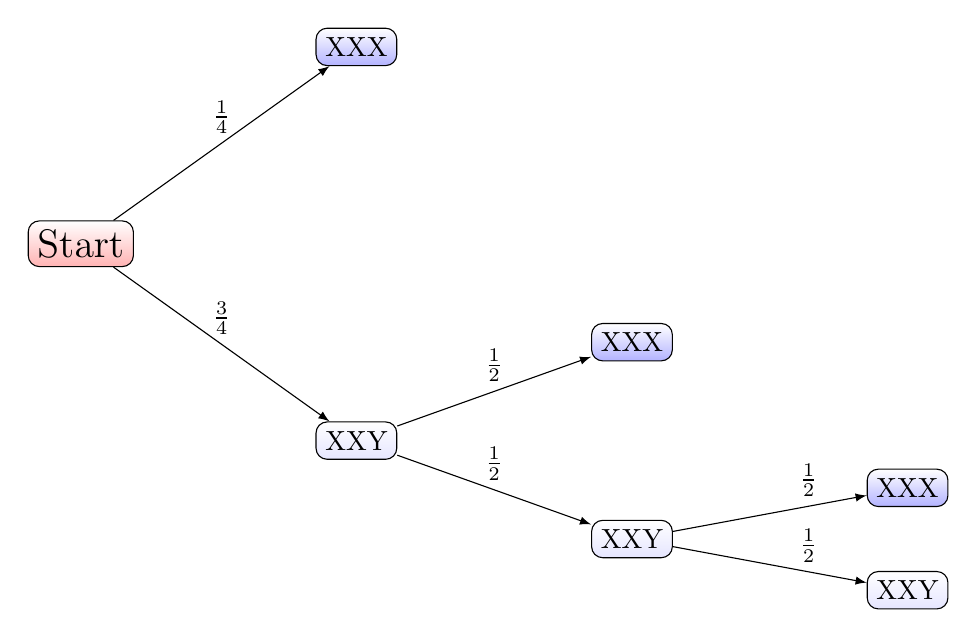
\begin{tikzpicture}
[
grow=right,
    edge from parent/.style = {draw, -latex},
    every node/.style       = {font=\normalsize}
  ]
\node[root]{Start}
child { 
    node[branch]{XXY}
    child { 
        node[branch]{XXY}
        child{ 
             node[branch]{XXY}
             edge from parent node[above,pos=0.7]{$\frac{1}{2}$}                    }
        child{ 
             node[env]{XXX}
             edge from parent node[above,pos=0.7]{$\frac{1}{2}$}      
             }               
        edge from parent node[above]{$\frac{1}{2}$} 
        }       
    child { 
        node[env]{XXX}             
        edge from parent node[above]{$\frac{1}{2}$} 
        }       
    edge from parent node[above]{$\frac{3}{4}$}            
    }
child { 
    node[env]{XXX} 
    edge from parent node[above]{$\frac{1}{4}$}            
    }     ;           
\end{tikzpicture}

From the tree, the probability of success occurring in round 1 is $1/4$, in round 2 it is $3/8$ and in round 3 it is $3/16$.  So your probability of having succeeded by the 1st round is $1/4$, by the second round is $5/8$ and by the 3rd round is $13/16$. 

In the case of 5 coins, your initial tree should have three branches: XXXXX, XXXXY and XXXYY. 
\end{s}

\sse 
Imagine a multiple test question having four options to choose between. In a simplified model we assume that for each student there is a probability $p$ that they know the answer in which case they certainly choose the correct option and if they do not know the answer they can only guess at random between the four options.  What is the probability that a student gets a question correct? 

In a test of 20 such questions, it is common practice to give a mark out of 15 which is equal to the number of correct answers minus 5. Does this seem reasonable? 
\end{e}

\sss
The probability of getting a question right by knowing the answer is $p$ and so the student does not know the answer with probability $1-p$. In the latter case, they get it right by guessing with probability $1/4$. So in total the probability of getting it right (draw a tree) is $p + (1-p)/4 = (3/4)p +(1/4)$. 

Thus in 20 questions it is expected that the student will score $15p+5$ marks.  One could therefore argue that a mark out of 15 equal to the number of correct answers minus 5 is reasonable. 
\end{s}


\ssp 
You are doing a multiple choice quiz where each question has 4 possible answers A,B,C,D to choose from. You have not worked on this subject, so your answers are going to be a complete guess for every question. 

There is a "give me a hint" option and it works like this. First you make a provisional choice of answer. 
Whether your guess is right or wrong, the computer then chooses 
uniformly at random one of the other three possibilities that is incorrect.  So, for example, you might provisionally choose D and it might tell you that answer A is definitely wrong. At that point you can stick to your original guess, D in this case, or switch to one of B or C (in which case, presumably you choose one of the two at random) before submitting your final answer. 

\begin{enumerate}
\item If you ignore the hints and stick with your original choice each time, what is the probability that you get a question correct?
\item If each time you switch your guess to one of the two other possibilities, what is what is the probability that you get a question correct?   
\end{enumerate}
\end{e}

\sss
If you stick with your original answer, the probability of getting it right is the probability that your original guess was right, which is $1/4$. 

If you switch, then you end up being wrong if your initial answer was right. On the other hand, if you were wrong initially then one of two answers that you might switch to is right and you will choose the correct one half the time. So the probability of success is 
 \[
 \PP(\text{first guess wrong}) \, \PP(\text{choosing correctly from two}) = \frac34 \, \frac12 = \frac38
 \]
 So switching increases your chance of being correct by 50\%. 
 (This is a modification of the famous ``Monty Hall problem''.) 
 
 
\end{s}


\ssp 
Consider the following game played with a collection of coins all of equal value.  Unseen by you, I choose to put either one coin or two in my hand and then ask you to guess whether I am holding one or two coins. If you are right, then you receive the coin(s). If you are wrong, you receive nothing.  

If I always choose the same option, you will take advantage of this and win all the time. If you always make the same guess, I will take advantage and you will always lose. 
\begin{enumerate}
\item Suppose each time I choose whether to offer one or two coins I do so independently and uniformly randomly. Suppose too that every time you guess you independently do the same. What is your expected gain playing this game? 
\item (\textbf{Challenge})  If you think I am choosing one coin with probability $p=1/2$ then it makes sense for you to guess there are two coins with a probability $r>1/2$ because of the greater reward. How should rational players choose $p$ and $r$? 
\end{enumerate}
\end{e}

\sss
\begin{enumerate}
\item This is another tree/table problem. There are four equally likely outcomes made of every combination of me choosing 1 or 2 coins and you guessing 1 or 2 coins. In two cases you lose, in one you win 1 coin and in the final one you win 2. So your expected gain is 
\[
 \frac14 0 + \frac14 0 + \frac14 1 + \frac14 2 = \frac34.
\]
\item This is a challenge. 
A good starting point is to evaluate your expected winnings if I choose 1 coin with probability $p$ and you guess 2 coins with probability $r$. 
\end{enumerate}
\end{s}





